% Copyright 2013 Nicolai Hähnle <nhaehnle@gmail.com>
%
% This work is licensed under the Creative Commons Attribution-ShareAlike 3.0
% Unported License, see http://creativecommons.org/licenses/by-sa/3.0/
%
% Among other things, this means that yes, you may take e.g. illustrations from
% the book and use them in your own work. However, (a) you must give proper
% attribution by naming me as its original author and (b) you must make your
% derivative work available under the same or similar license terms.
%
% See the Creative Commons website for the exact licensing terms.

\chapter{Arbitrary Norms and Enumeration of Lattice Points}

We have seen how to find shortest and closest vectors in a lattice
with respect to the Euclidean norm in time essentially $2^{O(d)}$,
ignoring some polynomial factors in the encoding size of the input.
What about the related problems with respect to an arbitrary norm $\|\cdot\|$?

In the decision variant of the closest vector problem,
we are given a lattice $\Lambda \subset \R^d$,
target vector $t \in \R^d$
and target distance $r > 0$,
and we have to decide whether there is a lattice point $x \in \Lambda$
with $\|x - t\| \leq r$.
This is a lattice programming problem:
decide whether the norm ball $B_{\|\cdot\|}(t,r)$ contains a lattice point.
We have seen that such problems can be solved in essentially
$2^{O(d \log d)}$ arithmetic operations
and calls to an oracle describing $B_{\|\cdot\|}(t,r)$
which we can derive from an oracle describing the norm $\|\cdot\|$.
There is a gap between this running time and
the time we could previously achieve for the Euclidean norm.

We do not know how to adapt the techniques based on Voronoi cells
since Voronoi diagrams in other norms are rather unwieldy.
For one thing, Voronoi cells are not convex in general!

A different approach is needed.
Suppose we could somehow enumerate the lattice points in any convex body efficiently,
by an output-sensitive algorithm,
in time $(N+1)\cdot 2^{O(d)}$
where $N$ is the number of lattice points that are found.

Then a natural algorithm for solving the shortest vector problem is as follows:
Start with a lower bound $r = r_0$ on the $\|\cdot\|$-length of a shortest vector
and enumerate lattice points in the $\|\cdot\|$-ball of radius $r$ around the origin.
If a non-zero lattice point is found, output the shortest among them.
Otherwise, multiply $r$ by a constant factor and repeat.

Due to a volume argument,
the first $\|\cdot\|$-ball to contain \emph{any} non-zero lattice points
can only contain $2^{O(d)}$ of them.
Then the overall running time is still bounded by a single-exponential factor
times the logarithm of the quality of the initial estimate $r_0$.

In this chapter,
we will visit some theory on arbitrary norms,
develop a lattice point enumeration algorithm,
and use it to solve the shortest vector problem
and approximate the closest vector problem
with respect to arbitrary norms.


\section{Norms and Convex Bodies}

The unit ball
$B_{\|\cdot\|}(0,1)$
with respect to an arbitrary norm $\|\cdot\|$
is a compact convex set of positive volume.
Furthermore, it is \emph{symmetric}
in the sense that $B_{\|\cdot\|}(0,1) = -B_{\|\cdot\|}(0,1)$.

\begin{definition}
  Let $K$ be a symmetric, compact, convex set of positive volume.
  We define the norm associated to $K$ as
  \[
    \| x \|_K := \min\{ r \geq 0 ~:~ x \in r K \}
  \]
\end{definition}
\begin{lemma}
  $\|\cdot\|_K$ is a norm.
\end{lemma}



\section{Enumerating lattice points in an ellipsoid}



\section{Some examples on enumeration}

Now that we can enumerate lattice points in an ellipsoid,
a natural idea for enumerating points in a more general body $K$
is to take an ellipsoid $E$ of smallest volume enclosing $K$.
However, this approach cannot lead to an efficient algorithm.

Consider the cube
\[
  P := [-1, +1]^d,
\]
whose smallest enclosing ellipsoid is the $\ell_2$ ball $B = B(0,\sqrt{d})$.
Let us place a cube


THE FOLLOWING IS INCORRECT!

Consider the cross-polytope
\[
  P := \conv\{ \pm e_j ~:~ 1 \leq j \leq d \}
\]
whose smallest enclosing ellipsoid is the $\ell_2$-unit ball $B = B(0,1)$:
\begin{center}
  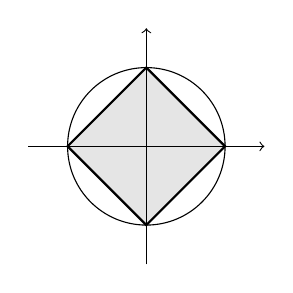
\begin{tikzpicture}
    \draw[thick,fill=black!10] (-1,0) -- (0,-1) -- (1,0) -- (0,1) --cycle;
    \draw[->] (-1.5,0) -- (1.5,0);
    \draw[->] (0,-1.5) -- (0,1.5);
    \draw (0,0) circle[radius=1cm];
  \end{tikzpicture}
\end{center}
Observe that $P^\star = [-1,+1]^d$
and so $P$ can be described by a system of $2^d$ inequalities:
\[
  P = \{ x \in \R^d ~:~ \pm x_1 \pm \dots \pm x_d \leq 1 \}
\]
Let $d$ be such that a Hadamard matrix $H \in \{ \pm 1 \}^{d \times d}$ exists.
Recall that a Hadamard matrix is a matrix with all entries either $+1$ or $-1$
such that the rows and columns are pairwise orthogonal.
It is easy to construct Hadamard matrices via a recursive construction
when $d$ is a power of $2$.

Consider the lattice $\Lambda := \frac{1}{d} \Lambda(H)$.
We claim that:
\begin{enumerate}
  \item $0$ is the only lattice point in the interior of $P$, and
  \item there are $2^{\Omega(d \log d)}$ lattice points in the interior of $B$.
\end{enumerate}
That is, enumeration of lattice points in the smallest enclosing ellipsoid of $P$
takes more than $(N+1)\cdot 2^{O(d)}$ time when $N$ is the number of lattice points found in $P$.

For the first claim,
let $x = \frac{\alpha_1}{d} h_1 + \dots + \frac{\alpha_d}{d} h_d \in \Lambda\setminus 0$.
Note that $\alpha_j \in \Z$.
Let $k$ be an index such that $\alpha_k \neq 0$.
Then
\[
  h_k^T x = \frac{\alpha_k}{d} h_k^T h_k = \alpha_k
\]
Since $h_k^Tx \leq 1$ and $-h_k^Tx \leq 1$ are valid inequalities for $P$,
this means that $x$ is not in the interior of $P$.

For the second claim,
first observe that the fundamental parallelepiped $\cP$ of $\Lambda$
is a cube with edge lengths $\|\frac{1}{d} h_j\| = 1/\sqrt{d}$.
Let us center a copy of $\cP$ around every lattice point in the interior of $B$,
see Figure~\ref{fig:hadamard-lattice-covering}.
Each copy of $\cP$ is contained in a ball of radius $1/2$,
and so the copies together cover the open ball of radius $1/2$.

\begin{figure}
  \begin{center}
    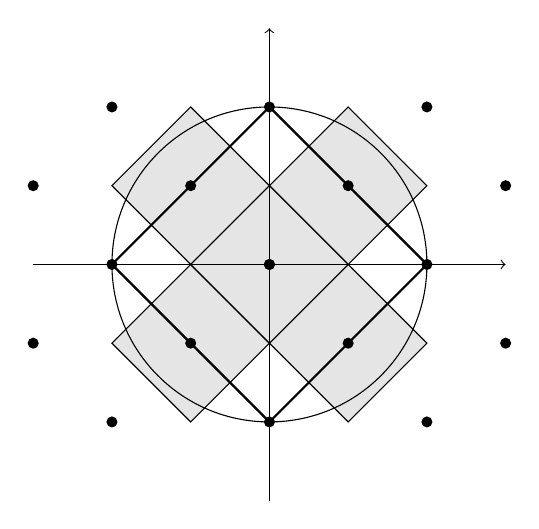
\begin{tikzpicture}
      \foreach \p in {
            (-1,-1),(1,-1),
            (0,0),
            (-1,1),(1,1),
        } {
        \draw[fill=black!10] \p +(-1,0) -- +(0,-1) -- +(1,0) -- +(0,1) -- cycle;
      }

      \draw[thick] (-2,0) -- (0,-2) -- (2,0) -- (0,2) --cycle;
      \draw[->] (-3,0) -- (3,0);
      \draw[->] (0,-3) -- (0,3);
      \draw (0,0) circle[radius=2cm];

      \foreach \p in {
            (-2,-2),(0,-2),(2,-2),
            (-3,-1),(-1,-1),(1,-1),(3,-1),
            (-2,0),(0,0),(2,0),
            (-3,1),(-1,1),(1,1),(3,1),
            (-2,2),(0,2),(2,2),
        } {
        \fill \p circle[radius=2pt];
      }
    \end{tikzpicture}
  \end{center}
  \caption{Lower bounding the number of lattice points in $B$
    with a volume argument.}
  \label{fig:hadamard-lattice-covering}
\end{figure}

Let $N$ be the number of lattice points in the interior of $B$.
We have
\[
  \vol B(0,\frac{1}{2}) \leq N \cdot \vol(\cP_B) = N \cdot \left(\frac{1}{\sqrt{d}}\right)^d
\]
